\section{State-based assertions on fluents\label{section:background-fluents}}

Miller and Shanahan define fluents as ``\emph{time-varying properties of the world that are true at particular time-points if they have been initiated by an event occurrence at some earlier time-point, and not terminated by another event occurrence in the meantime. Similarly, a fluent is false at a particular time-point if it has been previously terminated and not initiated in the meantime}''~\cite{Miller:2002}.

Fluents will allow us to integrate event-based and state-based specification styles within a simple framework~\cite{Giannakopoulou:2003}. A fluent $Fl$ is thus a proposition defined by a set $Init_{Fl}$ of initiating events, a set $Term_{Fl}$ of terminating events, and an initial value $Initially_{Fl}$ that can be true or false. The sets of initiating and terminating events must be disjoint. The concrete syntax for fluent definitions is the following~\cite{Giannakopoulou:2003}:

\begin{center}
fluent $Fl = \textless Init_{Fl}, Term_{Fl} \textgreater $ initially $Initially_{Fl}$
\end{center}

In our train example, the safety goal ``\emph{\texttt{Doors shall remain closed while the train is moving}}'' suggests two fluents defined as follows:

\begin{center}
fluent $Moving = \textless \{start\}, \{stop\} \textgreater $ initially $false$ \\
fluent $DoorsClosed = \textless \{close\}, \{open\} \textgreater $ initially $true$ \\
\end{center}

\subsection{Fluent values along single traces\label{subsection:background-fluents-single-traces}}

In terms of our trace semantics, a fluent $Fl$ will be $true$ after a finite trace $s$ if and only if one of the following conditions hold~\cite{Giannakopoulou:2003}:

\begin{enumerate}
\item $Fl$ holds initially and no terminating event has occurred in $s$.
\item Some initiating event has occurred in $s$ with no terminating event occurring since then.
\end{enumerate}

For example, the fluent $Moving$ is $true$ after the trace \artifact{<start stop start>}, but not after the empty trace $\lambda$ nor after \artifact{<start stop>}. 

As sets of initiating and terminating events are disjoint, the value of a fluent after a given trace is deterministic. We may also think in terms of fluent values \emph{along} traces by rephrasing the above definition into a recursive version~\cite{Damas:2005, Damas:2011}. This is illustrated in Fig.~\ref{image:fluent-values-along-a-trace} where the values of the two fluents given above are shown in the states of a LTS capturing a typical event trace for the train system. 

\begin{figure}[H]\centering
\scalebox{0.45}{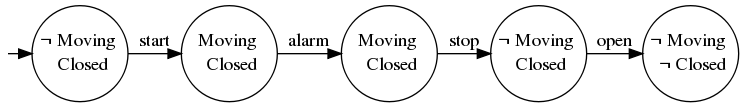
\includegraphics{src/2-framework/images/decorating-trace}}
\caption{LTS annotated with fluent values along a single trace (\artifact{Closed} is an abbreviate for \artifact{DoorsClosed}).\label{image:fluent-values-along-a-trace}}
\end{figure}

As the example suggests, for a set of fluents $\Phi$, an event trace yields an interpretation over $2^\Phi$, that is, an assignment of a Boolean values to each fluent in $\Phi$. We will call them \emph{fluent value assignments} throughout this thesis. 

For example, the maximal trace Fig. \ref{image:fluent-values-along-a-trace} yields the fluent value assignment $\{Moving \rightarrow false,~DoorsClosed \rightarrow false\}$. 

\subsection{Fluent values along multiple traces}

We can similarly annotate the states of any LTS. The generalization consists in considering that a LTS state may be reached by a set of traces instead of a single one. Annotations therefore become \emph{sets} of fluent assignments, that is elements of the powerset $\mathcal{P}(2^\Phi)$ over $2^\Phi$. In particular, a state might be reached by a trace yielding a fluent $true$, while another trace reaching it would yield the same fluent $false$. Note that even in presence of a possibly infinite number of traces, the set of all possible annotations is itself finite. Moreover, $\mathcal{P}(2^\Phi)$ actually coincides with the set of propositional formulas over fluents. In appears convenient to consider state annotations as such formulas, where $false$ then corresponds to an empty set of fluent assignments (i.e. an unreachable state) and \artifact{true} corresponds to the set of all possible assignments. Such state annotations will be called \emph{fluent invariants}; they encode assertions that always hold when the LTS state is visited. Fig.~\ref{image:fluent-values-along-multiple-traces} shows an example of LTS annotation with state invariants.

\begin{figure}[H]\centering
\scalebox{0.45}{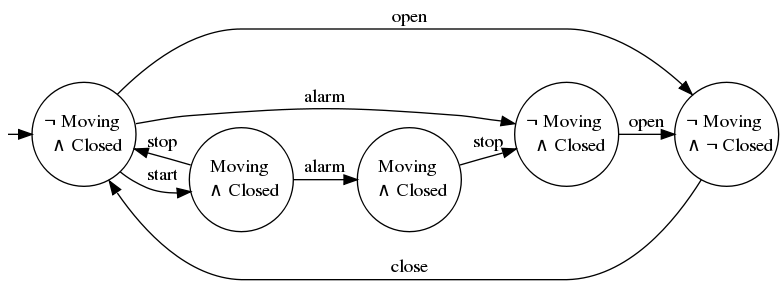
\includegraphics{src/2-framework/images/decorating-lts}}
\caption{Fluent values along multiple traces (\artifact{Closed} is an abbreviate for \artifact{DoorsClosed}.\label{image:fluent-values-along-multiple-traces}}
\end{figure}

A fix-point algorithm for decorating LTS with fluent assignments first appeared in~\cite{Damas:2005}. This algorithm was generalized for handling state invariants in \cite{Damas:2009, Damas:2011}. Roughly, it consists in annotating the LTS initial state with an initial invariant according to fluent initial values. Invariants are then propagated along LTS transitions, according to fluent definitions, and accumulated in states through Boolean disjunction until a fix point is reached. Binary decision diagrams~\cite{Bryant:1986} can be used for concisely encoding and efficiently manipulating Boolean formulas (see Chapter~\ref{chapter:tool-support}). This algorithm has been further generalized in~\cite{Damas:2011} for guarded LTS (see Chapter~\ref{chapter:deductive}) for handling other kinds of decorations than state invariants.

\subsection{Integrating fluents in multi-view models}

Fluents provide a general mechanism for integrating event-based and state-based specifications. This section restricts the use of this mechanism to cleanly integrate agents, their state machines, and scenarios. The next section extends this discussion by introducing fluent-based goals and domain properties in the framework.

We will restrict our use of fluents to the ones monitorable and controllable by the agents forming the system~\cite{Letier:2002}. 

A fluent is \emph{monitorable} by an agent if all its initiating and terminating events can be either sent or received by this agent. It is \emph{controllable} if all initiating and terminating events are sent by the agent. 

Our restriction to fluents that are monitorable or controllable by system agents is motivated by the need for specifications  to be realizable by the agents involved in them~\cite{Letier:2002}.

As seen in the previous section, the value of a fluent is not necessarily known in a LTS state because some traces could make it $true$ while others could make it $false$. While there is no strong agreement for viewing this as problematic in general, we consider a good practice not to fall in such a situation between the fluents monitored and controlled by an agent and the state machine modeling its behavior. The reason is that LTSs are not considered a structured form of state machines. Therefore, a LTS state should not be viewed as a class of agent states, that is, it should correspond to a unique assignment of agent state variables; fluents are such variables. The LTS state machine shown in Fig.~\ref{image:fluent-values-along-multiple-traces} meets this sane property. In particular, one can check that propositional formula shown in states are satisfiable by only one interpretation (fluent invariants ``degenerate'' to fluent value assignments). In such a case, an agent state uniquely defines the value of its monitored and controlled fluents (this property is conserved under LTS composition by construction). The contrapositive of this property is not true: as illustrated in the same figure, fluent value assignments do not necessarily identify LTS states.

In a similar way, MSC timelines can be annotated with agent invariants on monitorable and controllable fluents. Note again that such invariants do not necessarily identify agent states in a unique manner.
